The subject of the present work deals with the propagation, non-linear mixing effects of high-frequency shear and longitudinal waves which help us characterize material properties. This section is a brief introduction containing the background, outline and applications of the presented work.

\section{Background}
The stress-strain curve for most ductile materials starts in a linear relationship and moves into a non-linear relationship with a few invariants that define the said relationship. Determining these constants is of great use to characterize the material and predict its behaviour under various conditions and also optimize processes with respect to these constants. While the physical relationship between the linear constants and their estimation has been studied to a great extent, the non-linear constants are more difficult to estimate. Our work aims to estimate these non-linear constants through statistical estimation techniques.

\subsection{The stress-strain curve}
\begin{center}
\begin{figure}[ht]
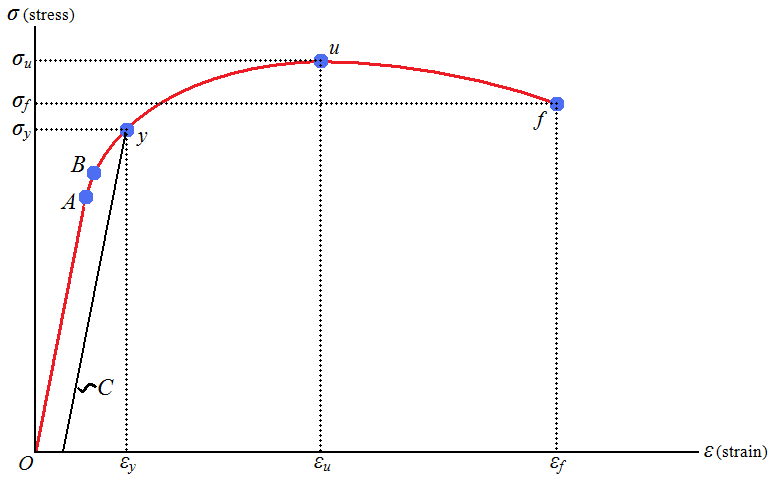
\includegraphics[scale=0.45]{images/chapter_1/stressstrain.png}
\caption{The Stress Strain Curve for a Typical Material}
\end{figure}
\end{center}
The significant points from fig 1.1.1 are as follows:
\begin{enumerate}
\item A - Proportional Limit
\item B - Elastic Limit
\item y - Yield Point
\item u - Ultimate Tensile Strength
\item f - Fracture point
\end{enumerate}
\subsection{Non-Destructive Testing}
There are multiple methods of figuring out the elastic constants of a material, most significant of them being destructive methods, where the material is stressed to its Ultimate Tensile Strength and then, a curve is fit to get the second order constants of the material. This results in the material specimen being destroyed and deemed useless. This method is good for laboratory conditions, but not in a real-world scenario.

To account for this, we employ a method of Non-Destructive testing using ultrasonics. Ultrasonic waves have the characteristic of extremely high strain rates, but the magnitude of strain itself is minimal, and the changes to material properties are thus negligible. These high strain rates result in interesting phenomenon occurring, which in turn helps us estimate parameters of the material, without any physical damage to the specimen.

\subsection{Wave Propagation and Mixing}
One of the main concepts that are used in this study are that of wave propagation in solid media and mixing of waves in linear and non-linear zones. To solve the differential equations involved, we use FDTD simulations. We employed multiple solvers to evaluate the equations and multiple approaches to solve the problem. This will be discussed in detail in upcoming chapters.

\subsection{Statistical Inversion and Learning}
The forward model is inverted by using purely statistical techniques. We employ various techniques from Support Vector Machines (SVM), Gaussian Mixture Models (GMMs), and Gaussian Processes. The mathematics and results will be discussed in detail in the coming chapters.
\section{Outline of the Report}
This report is organized into 6 chapters.
\begin{enumerate}

\item The current chapter gives a basic introduction to the project and explains very briefly what we hope to achieve and techniques we've employed with a little bit of background information.

\item Chapter 2 deals with Literature Review and what we worked on and the subsequent results of the same with reasons as to what method we finally adopted and why with a discussion about the same.

\item Chapter 3 describes the construction of the FDTD model for the forward problem and the collinear wave mixing approach that is taken by us and describes the problem and solution in detail.

\item Chapter 4 explores the sensitivity analysis of our constructed forward model with respect to various parameters of interest and and exploratory analysis of the inverse model.

\item Chapter 5 validates the inverse model and also describes the pitfalls of the model. We make the model more real world friendly and check its performance.

\item Chapter 6 summarizes our work and has a section on how this project can be pursued along with suggestions for experimental validation.
\end{enumerate}
\section{Applications of present work}
The present work has wide range of uses from aircraft industry to the shipping industry. A manufacturing specific application of this current technique will be in the estimation of material parameters in forming process and cold working processes where materials undergo plastic deformation. 

This technique will help us understand material deformation better and give us a physical insight into what the constants mean and at the same time help improve existing processes and diagnose issues in current processes.  